% Every number in this paper comes from ../results (see ../PROTOCOL.md, Section 8).
% Numbers in the text use \res{key}; keys are generated by scripts/07_paper_assets.py.
% An undefined key renders as a bold ??key?? so it cannot slip through silently.
\documentclass[sigconf,nonacm]{acmart}

\usepackage{booktabs}
\usepackage{graphicx}
\usepackage{microtype}
\usepackage{amsmath}

% Generated by scripts/07_paper_assets.py from results files. Do not edit by hand.
\makeatletter
\newcommand{\res}[1]{\@ifundefined{res@#1}{\textbf{??#1??}}{\csname res@#1\endcsname}}
\expandafter\def\csname res@binding-rho0.3\endcsname{94.3}
\expandafter\def\csname res@binding-rho0.5\endcsname{86.5}
\expandafter\def\csname res@binding-rho0.7\endcsname{70.8}
\expandafter\def\csname res@cmp-nn-baselines-pmax\endcsname{0.00052}
\expandafter\def\csname res@cmp-nn-baselines-sig\endcsname{12}
\expandafter\def\csname res@cmp-nn-baselines-total\endcsname{12}
\expandafter\def\csname res@cmp-nn-lgb-pmax\endcsname{0.0026}
\expandafter\def\csname res@cmp-nn-lgb-sig\endcsname{6}
\expandafter\def\csname res@cmp-nn-lgb-total\endcsname{6}
\expandafter\def\csname res@cmp-q09-baselines-pmax\endcsname{6.7e-49}
\expandafter\def\csname res@cmp-q09-baselines-sig\endcsname{24}
\expandafter\def\csname res@cmp-q09-baselines-total\endcsname{24}
\expandafter\def\csname res@cmp-tft-nhits-pmax\endcsname{1}
\expandafter\def\csname res@cmp-tft-nhits-sig\endcsname{1}
\expandafter\def\csname res@cmp-tft-nhits-total\endcsname{3}
\expandafter\def\csname res@data-campaigns\endcsname{414}
\expandafter\def\csname res@data-campaigns-total\endcsname{675}
\expandafter\def\csname res@data-eval-impressions\endcsname{4{,}197{,}856}
\expandafter\def\csname res@data-impressions\endcsname{16{,}468{,}027}
\expandafter\def\csname res@data-spend-share\endcsname{91.7}
\expandafter\def\csname res@data-test-episodes\endcsname{2{,}070}
\expandafter\def\csname res@even-rho0.3-bur\endcsname{93.8}
\expandafter\def\csname res@even-rho0.3-click\endcsname{0.993}
\expandafter\def\csname res@even-rho0.3-click-hi\endcsname{1.000}
\expandafter\def\csname res@even-rho0.3-click-lo\endcsname{0.987}
\expandafter\def\csname res@even-rho0.3-conv\endcsname{0.997}
\expandafter\def\csname res@even-rho0.3-early\endcsname{15.0}
\expandafter\def\csname res@even-rho0.3-pvi\endcsname{0.342}
\expandafter\def\csname res@even-rho0.5-bur\endcsname{90.2}
\expandafter\def\csname res@even-rho0.5-click\endcsname{0.960}
\expandafter\def\csname res@even-rho0.5-click-hi\endcsname{0.967}
\expandafter\def\csname res@even-rho0.5-click-lo\endcsname{0.954}
\expandafter\def\csname res@even-rho0.5-conv\endcsname{0.966}
\expandafter\def\csname res@even-rho0.5-early\endcsname{6.4}
\expandafter\def\csname res@even-rho0.5-pvi\endcsname{0.314}
\expandafter\def\csname res@even-rho0.7-bur\endcsname{84.8}
\expandafter\def\csname res@even-rho0.7-click\endcsname{0.942}
\expandafter\def\csname res@even-rho0.7-click-hi\endcsname{0.950}
\expandafter\def\csname res@even-rho0.7-click-lo\endcsname{0.935}
\expandafter\def\csname res@even-rho0.7-conv\endcsname{0.946}
\expandafter\def\csname res@even-rho0.7-early\endcsname{2.8}
\expandafter\def\csname res@even-rho0.7-pvi\endcsname{0.261}
\expandafter\def\csname res@fc-early-max\endcsname{6.1}
\expandafter\def\csname res@fc-early-min\endcsname{3.4}
\expandafter\def\csname res@fc-lightgbm-cov80\endcsname{71.7}
\expandafter\def\csname res@fc-lightgbm-cross\endcsname{0.92}
\expandafter\def\csname res@fc-lightgbm-mase\endcsname{0.853}
\expandafter\def\csname res@fc-lightgbm-mase-sd\endcsname{0.000}
\expandafter\def\csname res@fc-lightgbm-mase-step1\endcsname{0.810}
\expandafter\def\csname res@fc-lightgbm-mase-step24\endcsname{0.871}
\expandafter\def\csname res@fc-lightgbm-medmase\endcsname{0.722}
\expandafter\def\csname res@fc-lightgbm-spl0.1\endcsname{0.080}
\expandafter\def\csname res@fc-lightgbm-spl0.5\endcsname{0.246}
\expandafter\def\csname res@fc-lightgbm-spl0.9\endcsname{0.185}
\expandafter\def\csname res@fc-naive-cov80\endcsname{60.6}
\expandafter\def\csname res@fc-naive-cross\endcsname{0.00}
\expandafter\def\csname res@fc-naive-mase\endcsname{0.917}
\expandafter\def\csname res@fc-naive-mase-sd\endcsname{0.000}
\expandafter\def\csname res@fc-naive-mase-step1\endcsname{0.920}
\expandafter\def\csname res@fc-naive-mase-step24\endcsname{0.908}
\expandafter\def\csname res@fc-naive-medmase\endcsname{0.793}
\expandafter\def\csname res@fc-naive-spl0.1\endcsname{0.095}
\expandafter\def\csname res@fc-naive-spl0.5\endcsname{0.262}
\expandafter\def\csname res@fc-naive-spl0.9\endcsname{0.194}
\expandafter\def\csname res@fc-nhits-cov80\endcsname{75.8}
\expandafter\def\csname res@fc-nhits-cross\endcsname{0.47}
\expandafter\def\csname res@fc-nhits-mase\endcsname{0.794}
\expandafter\def\csname res@fc-nhits-mase-sd\endcsname{0.014}
\expandafter\def\csname res@fc-nhits-mase-step1\endcsname{0.719}
\expandafter\def\csname res@fc-nhits-mase-step24\endcsname{0.813}
\expandafter\def\csname res@fc-nhits-medmase\endcsname{0.723}
\expandafter\def\csname res@fc-nhits-spl0.1\endcsname{0.078}
\expandafter\def\csname res@fc-nhits-spl0.5\endcsname{0.231}
\expandafter\def\csname res@fc-nhits-spl0.9\endcsname{0.158}
\expandafter\def\csname res@fc-pvi-max\endcsname{0.12}
\expandafter\def\csname res@fc-pvi-min\endcsname{0.08}
\expandafter\def\csname res@fc-tft-cov80\endcsname{76.9}
\expandafter\def\csname res@fc-tft-cross\endcsname{0.03}
\expandafter\def\csname res@fc-tft-mase\endcsname{0.787}
\expandafter\def\csname res@fc-tft-mase-sd\endcsname{0.004}
\expandafter\def\csname res@fc-tft-mase-step1\endcsname{0.729}
\expandafter\def\csname res@fc-tft-mase-step24\endcsname{0.814}
\expandafter\def\csname res@fc-tft-medmase\endcsname{0.708}
\expandafter\def\csname res@fc-tft-spl0.1\endcsname{0.076}
\expandafter\def\csname res@fc-tft-spl0.5\endcsname{0.229}
\expandafter\def\csname res@fc-tft-spl0.9\endcsname{0.161}
\expandafter\def\csname res@gain-even-max\endcsname{5.4}
\expandafter\def\csname res@gain-even-min\endcsname{3.4}
\expandafter\def\csname res@gain-pid-max\endcsname{2.0}
\expandafter\def\csname res@gain-pid-min\endcsname{0.7}
\expandafter\def\csname res@hedge-bur-max\endcsname{82.8}
\expandafter\def\csname res@hedge-bur-min\endcsname{75.2}
\expandafter\def\csname res@hedge-cost-max\endcsname{10.6}
\expandafter\def\csname res@hedge-cost-min\endcsname{7.7}
\expandafter\def\csname res@hedge-early-max\endcsname{0.7}
\expandafter\def\csname res@hedge-early-min\endcsname{0.1}
\expandafter\def\csname res@hindsight-rho0.3-bur\endcsname{90.4}
\expandafter\def\csname res@hindsight-rho0.3-click\endcsname{1.000}
\expandafter\def\csname res@hindsight-rho0.3-click-hi\endcsname{1.000}
\expandafter\def\csname res@hindsight-rho0.3-click-lo\endcsname{1.000}
\expandafter\def\csname res@hindsight-rho0.3-conv\endcsname{1.000}
\expandafter\def\csname res@hindsight-rho0.3-early\endcsname{13.4}
\expandafter\def\csname res@hindsight-rho0.3-pvi\endcsname{0.000}
\expandafter\def\csname res@hindsight-rho0.5-bur\endcsname{90.6}
\expandafter\def\csname res@hindsight-rho0.5-click\endcsname{1.000}
\expandafter\def\csname res@hindsight-rho0.5-click-hi\endcsname{1.000}
\expandafter\def\csname res@hindsight-rho0.5-click-lo\endcsname{1.000}
\expandafter\def\csname res@hindsight-rho0.5-conv\endcsname{1.000}
\expandafter\def\csname res@hindsight-rho0.5-early\endcsname{9.5}
\expandafter\def\csname res@hindsight-rho0.5-pvi\endcsname{0.000}
\expandafter\def\csname res@hindsight-rho0.7-bur\endcsname{87.8}
\expandafter\def\csname res@hindsight-rho0.7-click\endcsname{1.000}
\expandafter\def\csname res@hindsight-rho0.7-click-hi\endcsname{1.000}
\expandafter\def\csname res@hindsight-rho0.7-click-lo\endcsname{1.000}
\expandafter\def\csname res@hindsight-rho0.7-conv\endcsname{1.000}
\expandafter\def\csname res@hindsight-rho0.7-early\endcsname{6.0}
\expandafter\def\csname res@hindsight-rho0.7-pvi\endcsname{0.000}
\expandafter\def\csname res@lightgbm-q0.5-rho0.3-bur\endcsname{94.6}
\expandafter\def\csname res@lightgbm-q0.5-rho0.3-click\endcsname{1.019}
\expandafter\def\csname res@lightgbm-q0.5-rho0.3-click-hi\endcsname{1.024}
\expandafter\def\csname res@lightgbm-q0.5-rho0.3-click-lo\endcsname{1.013}
\expandafter\def\csname res@lightgbm-q0.5-rho0.3-conv\endcsname{1.013}
\expandafter\def\csname res@lightgbm-q0.5-rho0.3-early\endcsname{5.6}
\expandafter\def\csname res@lightgbm-q0.5-rho0.3-pvi\endcsname{0.094}
\expandafter\def\csname res@lightgbm-q0.5-rho0.5-bur\endcsname{92.4}
\expandafter\def\csname res@lightgbm-q0.5-rho0.5-click\endcsname{0.997}
\expandafter\def\csname res@lightgbm-q0.5-rho0.5-click-hi\endcsname{1.003}
\expandafter\def\csname res@lightgbm-q0.5-rho0.5-click-lo\endcsname{0.989}
\expandafter\def\csname res@lightgbm-q0.5-rho0.5-conv\endcsname{0.998}
\expandafter\def\csname res@lightgbm-q0.5-rho0.5-early\endcsname{5.0}
\expandafter\def\csname res@lightgbm-q0.5-rho0.5-pvi\endcsname{0.094}
\expandafter\def\csname res@lightgbm-q0.5-rho0.7-bur\endcsname{88.5}
\expandafter\def\csname res@lightgbm-q0.5-rho0.7-click\endcsname{0.992}
\expandafter\def\csname res@lightgbm-q0.5-rho0.7-click-hi\endcsname{0.995}
\expandafter\def\csname res@lightgbm-q0.5-rho0.7-click-lo\endcsname{0.989}
\expandafter\def\csname res@lightgbm-q0.5-rho0.7-conv\endcsname{0.996}
\expandafter\def\csname res@lightgbm-q0.5-rho0.7-early\endcsname{4.7}
\expandafter\def\csname res@lightgbm-q0.5-rho0.7-pvi\endcsname{0.083}
\expandafter\def\csname res@lightgbm-q0.7-rho0.3-bur\endcsname{91.1}
\expandafter\def\csname res@lightgbm-q0.7-rho0.3-click\endcsname{0.995}
\expandafter\def\csname res@lightgbm-q0.7-rho0.3-click-hi\endcsname{1.002}
\expandafter\def\csname res@lightgbm-q0.7-rho0.3-click-lo\endcsname{0.989}
\expandafter\def\csname res@lightgbm-q0.7-rho0.3-conv\endcsname{0.984}
\expandafter\def\csname res@lightgbm-q0.7-rho0.3-early\endcsname{1.8}
\expandafter\def\csname res@lightgbm-q0.7-rho0.3-pvi\endcsname{0.088}
\expandafter\def\csname res@lightgbm-q0.7-rho0.5-bur\endcsname{88.7}
\expandafter\def\csname res@lightgbm-q0.7-rho0.5-click\endcsname{0.972}
\expandafter\def\csname res@lightgbm-q0.7-rho0.5-click-hi\endcsname{0.979}
\expandafter\def\csname res@lightgbm-q0.7-rho0.5-click-lo\endcsname{0.964}
\expandafter\def\csname res@lightgbm-q0.7-rho0.5-conv\endcsname{0.964}
\expandafter\def\csname res@lightgbm-q0.7-rho0.5-early\endcsname{1.6}
\expandafter\def\csname res@lightgbm-q0.7-rho0.5-pvi\endcsname{0.082}
\expandafter\def\csname res@lightgbm-q0.7-rho0.7-bur\endcsname{85.0}
\expandafter\def\csname res@lightgbm-q0.7-rho0.7-click\endcsname{0.965}
\expandafter\def\csname res@lightgbm-q0.7-rho0.7-click-hi\endcsname{0.969}
\expandafter\def\csname res@lightgbm-q0.7-rho0.7-click-lo\endcsname{0.960}
\expandafter\def\csname res@lightgbm-q0.7-rho0.7-conv\endcsname{0.964}
\expandafter\def\csname res@lightgbm-q0.7-rho0.7-early\endcsname{1.6}
\expandafter\def\csname res@lightgbm-q0.7-rho0.7-pvi\endcsname{0.071}
\expandafter\def\csname res@lightgbm-q0.9-rho0.3-bur\endcsname{80.8}
\expandafter\def\csname res@lightgbm-q0.9-rho0.3-click\endcsname{0.914}
\expandafter\def\csname res@lightgbm-q0.9-rho0.3-click-hi\endcsname{0.926}
\expandafter\def\csname res@lightgbm-q0.9-rho0.3-click-lo\endcsname{0.900}
\expandafter\def\csname res@lightgbm-q0.9-rho0.3-conv\endcsname{0.896}
\expandafter\def\csname res@lightgbm-q0.9-rho0.3-early\endcsname{0.5}
\expandafter\def\csname res@lightgbm-q0.9-rho0.3-pvi\endcsname{0.082}
\expandafter\def\csname res@lightgbm-q0.9-rho0.5-bur\endcsname{78.2}
\expandafter\def\csname res@lightgbm-q0.9-rho0.5-click\endcsname{0.892}
\expandafter\def\csname res@lightgbm-q0.9-rho0.5-click-hi\endcsname{0.905}
\expandafter\def\csname res@lightgbm-q0.9-rho0.5-click-lo\endcsname{0.877}
\expandafter\def\csname res@lightgbm-q0.9-rho0.5-conv\endcsname{0.879}
\expandafter\def\csname res@lightgbm-q0.9-rho0.5-early\endcsname{0.5}
\expandafter\def\csname res@lightgbm-q0.9-rho0.5-pvi\endcsname{0.071}
\expandafter\def\csname res@lightgbm-q0.9-rho0.7-bur\endcsname{75.2}
\expandafter\def\csname res@lightgbm-q0.9-rho0.7-click\endcsname{0.887}
\expandafter\def\csname res@lightgbm-q0.9-rho0.7-click-hi\endcsname{0.895}
\expandafter\def\csname res@lightgbm-q0.9-rho0.7-click-lo\endcsname{0.877}
\expandafter\def\csname res@lightgbm-q0.9-rho0.7-conv\endcsname{0.880}
\expandafter\def\csname res@lightgbm-q0.9-rho0.7-early\endcsname{0.4}
\expandafter\def\csname res@lightgbm-q0.9-rho0.7-pvi\endcsname{0.060}
\expandafter\def\csname res@n-bootstrap\endcsname{2{,}000}
\expandafter\def\csname res@n-campaigns-paired\endcsname{409}
\expandafter\def\csname res@n-comparisons\endcsname{126}
\expandafter\def\csname res@n-nn-seeds\endcsname{3}
\expandafter\def\csname res@n-replay-seeds\endcsname{10}
\expandafter\def\csname res@n-significant\endcsname{103}
\expandafter\def\csname res@naive-q0.5-rho0.3-bur\endcsname{93.4}
\expandafter\def\csname res@naive-q0.5-rho0.3-click\endcsname{1.007}
\expandafter\def\csname res@naive-q0.5-rho0.3-click-hi\endcsname{1.014}
\expandafter\def\csname res@naive-q0.5-rho0.3-click-lo\endcsname{0.999}
\expandafter\def\csname res@naive-q0.5-rho0.3-conv\endcsname{1.000}
\expandafter\def\csname res@naive-q0.5-rho0.3-early\endcsname{6.6}
\expandafter\def\csname res@naive-q0.5-rho0.3-pvi\endcsname{0.087}
\expandafter\def\csname res@naive-q0.5-rho0.5-bur\endcsname{91.3}
\expandafter\def\csname res@naive-q0.5-rho0.5-click\endcsname{0.989}
\expandafter\def\csname res@naive-q0.5-rho0.5-click-hi\endcsname{0.994}
\expandafter\def\csname res@naive-q0.5-rho0.5-click-lo\endcsname{0.984}
\expandafter\def\csname res@naive-q0.5-rho0.5-conv\endcsname{0.988}
\expandafter\def\csname res@naive-q0.5-rho0.5-early\endcsname{6.4}
\expandafter\def\csname res@naive-q0.5-rho0.5-pvi\endcsname{0.083}
\expandafter\def\csname res@naive-q0.5-rho0.7-bur\endcsname{87.6}
\expandafter\def\csname res@naive-q0.5-rho0.7-click\endcsname{0.983}
\expandafter\def\csname res@naive-q0.5-rho0.7-click-hi\endcsname{0.987}
\expandafter\def\csname res@naive-q0.5-rho0.7-click-lo\endcsname{0.979}
\expandafter\def\csname res@naive-q0.5-rho0.7-conv\endcsname{0.986}
\expandafter\def\csname res@naive-q0.5-rho0.7-early\endcsname{5.9}
\expandafter\def\csname res@naive-q0.5-rho0.7-pvi\endcsname{0.071}
\expandafter\def\csname res@naive-q0.7-rho0.3-bur\endcsname{89.9}
\expandafter\def\csname res@naive-q0.7-rho0.3-click\endcsname{0.984}
\expandafter\def\csname res@naive-q0.7-rho0.3-click-hi\endcsname{0.992}
\expandafter\def\csname res@naive-q0.7-rho0.3-click-lo\endcsname{0.973}
\expandafter\def\csname res@naive-q0.7-rho0.3-conv\endcsname{0.969}
\expandafter\def\csname res@naive-q0.7-rho0.3-early\endcsname{2.6}
\expandafter\def\csname res@naive-q0.7-rho0.3-pvi\endcsname{0.083}
\expandafter\def\csname res@naive-q0.7-rho0.5-bur\endcsname{87.7}
\expandafter\def\csname res@naive-q0.7-rho0.5-click\endcsname{0.965}
\expandafter\def\csname res@naive-q0.7-rho0.5-click-hi\endcsname{0.972}
\expandafter\def\csname res@naive-q0.7-rho0.5-click-lo\endcsname{0.958}
\expandafter\def\csname res@naive-q0.7-rho0.5-conv\endcsname{0.957}
\expandafter\def\csname res@naive-q0.7-rho0.5-early\endcsname{2.4}
\expandafter\def\csname res@naive-q0.7-rho0.5-pvi\endcsname{0.075}
\expandafter\def\csname res@naive-q0.7-rho0.7-bur\endcsname{84.2}
\expandafter\def\csname res@naive-q0.7-rho0.7-click\endcsname{0.959}
\expandafter\def\csname res@naive-q0.7-rho0.7-click-hi\endcsname{0.965}
\expandafter\def\csname res@naive-q0.7-rho0.7-click-lo\endcsname{0.953}
\expandafter\def\csname res@naive-q0.7-rho0.7-conv\endcsname{0.958}
\expandafter\def\csname res@naive-q0.7-rho0.7-early\endcsname{2.2}
\expandafter\def\csname res@naive-q0.7-rho0.7-pvi\endcsname{0.062}
\expandafter\def\csname res@naive-q0.9-rho0.3-bur\endcsname{82.0}
\expandafter\def\csname res@naive-q0.9-rho0.3-click\endcsname{0.930}
\expandafter\def\csname res@naive-q0.9-rho0.3-click-hi\endcsname{0.942}
\expandafter\def\csname res@naive-q0.9-rho0.3-click-lo\endcsname{0.913}
\expandafter\def\csname res@naive-q0.9-rho0.3-conv\endcsname{0.911}
\expandafter\def\csname res@naive-q0.9-rho0.3-early\endcsname{0.7}
\expandafter\def\csname res@naive-q0.9-rho0.3-pvi\endcsname{0.082}
\expandafter\def\csname res@naive-q0.9-rho0.5-bur\endcsname{79.6}
\expandafter\def\csname res@naive-q0.9-rho0.5-click\endcsname{0.910}
\expandafter\def\csname res@naive-q0.9-rho0.5-click-hi\endcsname{0.921}
\expandafter\def\csname res@naive-q0.9-rho0.5-click-lo\endcsname{0.898}
\expandafter\def\csname res@naive-q0.9-rho0.5-conv\endcsname{0.897}
\expandafter\def\csname res@naive-q0.9-rho0.5-early\endcsname{0.6}
\expandafter\def\csname res@naive-q0.9-rho0.5-pvi\endcsname{0.070}
\expandafter\def\csname res@naive-q0.9-rho0.7-bur\endcsname{76.4}
\expandafter\def\csname res@naive-q0.9-rho0.7-click\endcsname{0.904}
\expandafter\def\csname res@naive-q0.9-rho0.7-click-hi\endcsname{0.914}
\expandafter\def\csname res@naive-q0.9-rho0.7-click-lo\endcsname{0.892}
\expandafter\def\csname res@naive-q0.9-rho0.7-conv\endcsname{0.898}
\expandafter\def\csname res@naive-q0.9-rho0.7-early\endcsname{0.4}
\expandafter\def\csname res@naive-q0.9-rho0.7-pvi\endcsname{0.058}
\expandafter\def\csname res@nhits-q0.5-rho0.3-bur\endcsname{94.8}
\expandafter\def\csname res@nhits-q0.5-rho0.3-click\endcsname{1.028}
\expandafter\def\csname res@nhits-q0.5-rho0.3-click-hi\endcsname{1.033}
\expandafter\def\csname res@nhits-q0.5-rho0.3-click-lo\endcsname{1.024}
\expandafter\def\csname res@nhits-q0.5-rho0.3-conv\endcsname{1.022}
\expandafter\def\csname res@nhits-q0.5-rho0.3-early\endcsname{5.2}
\expandafter\def\csname res@nhits-q0.5-rho0.3-pvi\endcsname{0.118}
\expandafter\def\csname res@nhits-q0.5-rho0.5-bur\endcsname{92.5}
\expandafter\def\csname res@nhits-q0.5-rho0.5-click\endcsname{1.007}
\expandafter\def\csname res@nhits-q0.5-rho0.5-click-hi\endcsname{1.010}
\expandafter\def\csname res@nhits-q0.5-rho0.5-click-lo\endcsname{1.004}
\expandafter\def\csname res@nhits-q0.5-rho0.5-conv\endcsname{1.005}
\expandafter\def\csname res@nhits-q0.5-rho0.5-early\endcsname{4.3}
\expandafter\def\csname res@nhits-q0.5-rho0.5-pvi\endcsname{0.118}
\expandafter\def\csname res@nhits-q0.5-rho0.7-bur\endcsname{88.3}
\expandafter\def\csname res@nhits-q0.5-rho0.7-click\endcsname{0.995}
\expandafter\def\csname res@nhits-q0.5-rho0.7-click-hi\endcsname{0.998}
\expandafter\def\csname res@nhits-q0.5-rho0.7-click-lo\endcsname{0.992}
\expandafter\def\csname res@nhits-q0.5-rho0.7-conv\endcsname{0.996}
\expandafter\def\csname res@nhits-q0.5-rho0.7-early\endcsname{3.4}
\expandafter\def\csname res@nhits-q0.5-rho0.7-pvi\endcsname{0.101}
\expandafter\def\csname res@nhits-q0.7-rho0.3-bur\endcsname{91.7}
\expandafter\def\csname res@nhits-q0.7-rho0.3-click\endcsname{1.011}
\expandafter\def\csname res@nhits-q0.7-rho0.3-click-hi\endcsname{1.016}
\expandafter\def\csname res@nhits-q0.7-rho0.3-click-lo\endcsname{1.007}
\expandafter\def\csname res@nhits-q0.7-rho0.3-conv\endcsname{0.997}
\expandafter\def\csname res@nhits-q0.7-rho0.3-early\endcsname{1.5}
\expandafter\def\csname res@nhits-q0.7-rho0.3-pvi\endcsname{0.104}
\expandafter\def\csname res@nhits-q0.7-rho0.5-bur\endcsname{89.1}
\expandafter\def\csname res@nhits-q0.7-rho0.5-click\endcsname{0.985}
\expandafter\def\csname res@nhits-q0.7-rho0.5-click-hi\endcsname{0.989}
\expandafter\def\csname res@nhits-q0.7-rho0.5-click-lo\endcsname{0.981}
\expandafter\def\csname res@nhits-q0.7-rho0.5-conv\endcsname{0.976}
\expandafter\def\csname res@nhits-q0.7-rho0.5-early\endcsname{1.1}
\expandafter\def\csname res@nhits-q0.7-rho0.5-pvi\endcsname{0.101}
\expandafter\def\csname res@nhits-q0.7-rho0.7-bur\endcsname{84.9}
\expandafter\def\csname res@nhits-q0.7-rho0.7-click\endcsname{0.971}
\expandafter\def\csname res@nhits-q0.7-rho0.7-click-hi\endcsname{0.975}
\expandafter\def\csname res@nhits-q0.7-rho0.7-click-lo\endcsname{0.967}
\expandafter\def\csname res@nhits-q0.7-rho0.7-conv\endcsname{0.967}
\expandafter\def\csname res@nhits-q0.7-rho0.7-early\endcsname{0.9}
\expandafter\def\csname res@nhits-q0.7-rho0.7-pvi\endcsname{0.088}
\expandafter\def\csname res@nhits-q0.9-rho0.3-bur\endcsname{82.8}
\expandafter\def\csname res@nhits-q0.9-rho0.3-click\endcsname{0.950}
\expandafter\def\csname res@nhits-q0.9-rho0.3-click-hi\endcsname{0.957}
\expandafter\def\csname res@nhits-q0.9-rho0.3-click-lo\endcsname{0.941}
\expandafter\def\csname res@nhits-q0.9-rho0.3-conv\endcsname{0.928}
\expandafter\def\csname res@nhits-q0.9-rho0.3-early\endcsname{0.2}
\expandafter\def\csname res@nhits-q0.9-rho0.3-pvi\endcsname{0.095}
\expandafter\def\csname res@nhits-q0.9-rho0.5-bur\endcsname{79.6}
\expandafter\def\csname res@nhits-q0.9-rho0.5-click\endcsname{0.919}
\expandafter\def\csname res@nhits-q0.9-rho0.5-click-hi\endcsname{0.927}
\expandafter\def\csname res@nhits-q0.9-rho0.5-click-lo\endcsname{0.911}
\expandafter\def\csname res@nhits-q0.9-rho0.5-conv\endcsname{0.904}
\expandafter\def\csname res@nhits-q0.9-rho0.5-early\endcsname{0.2}
\expandafter\def\csname res@nhits-q0.9-rho0.5-pvi\endcsname{0.087}
\expandafter\def\csname res@nhits-q0.9-rho0.7-bur\endcsname{75.6}
\expandafter\def\csname res@nhits-q0.9-rho0.7-click\endcsname{0.904}
\expandafter\def\csname res@nhits-q0.9-rho0.7-click-hi\endcsname{0.913}
\expandafter\def\csname res@nhits-q0.9-rho0.7-click-lo\endcsname{0.894}
\expandafter\def\csname res@nhits-q0.9-rho0.7-conv\endcsname{0.894}
\expandafter\def\csname res@nhits-q0.9-rho0.7-early\endcsname{0.1}
\expandafter\def\csname res@nhits-q0.9-rho0.7-pvi\endcsname{0.078}
\expandafter\def\csname res@nn-lgb-max\endcsname{1.0}
\expandafter\def\csname res@nn-lgb-min\endcsname{0.3}
\expandafter\def\csname res@nn-naive-max\endcsname{2.1}
\expandafter\def\csname res@nn-naive-min\endcsname{1.2}
\expandafter\def\csname res@nopacing-conv-max\endcsname{3.2}
\expandafter\def\csname res@nopacing-conv-min\endcsname{1.4}
\expandafter\def\csname res@nopacing-early-max\endcsname{92.1}
\expandafter\def\csname res@nopacing-early-min\endcsname{59.1}
\expandafter\def\csname res@nopacing-rho0.3-bur\endcsname{96.8}
\expandafter\def\csname res@nopacing-rho0.3-click\endcsname{0.985}
\expandafter\def\csname res@nopacing-rho0.3-click-hi\endcsname{0.993}
\expandafter\def\csname res@nopacing-rho0.3-click-lo\endcsname{0.977}
\expandafter\def\csname res@nopacing-rho0.3-conv\endcsname{1.032}
\expandafter\def\csname res@nopacing-rho0.3-early\endcsname{92.1}
\expandafter\def\csname res@nopacing-rho0.3-pvi\endcsname{0.000}
\expandafter\def\csname res@nopacing-rho0.5-bur\endcsname{94.4}
\expandafter\def\csname res@nopacing-rho0.5-click\endcsname{0.979}
\expandafter\def\csname res@nopacing-rho0.5-click-hi\endcsname{0.986}
\expandafter\def\csname res@nopacing-rho0.5-click-lo\endcsname{0.973}
\expandafter\def\csname res@nopacing-rho0.5-conv\endcsname{1.018}
\expandafter\def\csname res@nopacing-rho0.5-early\endcsname{80.1}
\expandafter\def\csname res@nopacing-rho0.5-pvi\endcsname{0.000}
\expandafter\def\csname res@nopacing-rho0.7-bur\endcsname{90.1}
\expandafter\def\csname res@nopacing-rho0.7-click\endcsname{0.988}
\expandafter\def\csname res@nopacing-rho0.7-click-hi\endcsname{0.992}
\expandafter\def\csname res@nopacing-rho0.7-click-lo\endcsname{0.983}
\expandafter\def\csname res@nopacing-rho0.7-conv\endcsname{1.014}
\expandafter\def\csname res@nopacing-rho0.7-early\endcsname{59.1}
\expandafter\def\csname res@nopacing-rho0.7-pvi\endcsname{0.000}
\expandafter\def\csname res@pid-early-max\endcsname{31.9}
\expandafter\def\csname res@pid-early-min\endcsname{12.8}
\expandafter\def\csname res@pid-gains-rho0.3\endcsname{$K_p{=}16, K_i{=}0, K_d{=}32$}
\expandafter\def\csname res@pid-gains-rho0.5\endcsname{$K_p{=}0.03125, K_i{=}1, K_d{=}32$}
\expandafter\def\csname res@pid-gains-rho0.7\endcsname{$K_p{=}0.125, K_i{=}1, K_d{=}32$}
\expandafter\def\csname res@pid-pvi-max\endcsname{0.60}
\expandafter\def\csname res@pid-pvi-min\endcsname{0.43}
\expandafter\def\csname res@pid-rho0.3-bur\endcsname{94.8}
\expandafter\def\csname res@pid-rho0.3-click\endcsname{1.009}
\expandafter\def\csname res@pid-rho0.3-click-hi\endcsname{1.016}
\expandafter\def\csname res@pid-rho0.3-click-lo\endcsname{1.002}
\expandafter\def\csname res@pid-rho0.3-conv\endcsname{1.011}
\expandafter\def\csname res@pid-rho0.3-early\endcsname{12.8}
\expandafter\def\csname res@pid-rho0.3-pvi\endcsname{0.599}
\expandafter\def\csname res@pid-rho0.5-bur\endcsname{92.2}
\expandafter\def\csname res@pid-rho0.5-click\endcsname{0.990}
\expandafter\def\csname res@pid-rho0.5-click-hi\endcsname{0.996}
\expandafter\def\csname res@pid-rho0.5-click-lo\endcsname{0.983}
\expandafter\def\csname res@pid-rho0.5-conv\endcsname{1.004}
\expandafter\def\csname res@pid-rho0.5-early\endcsname{31.9}
\expandafter\def\csname res@pid-rho0.5-pvi\endcsname{0.577}
\expandafter\def\csname res@pid-rho0.7-bur\endcsname{87.8}
\expandafter\def\csname res@pid-rho0.7-click\endcsname{0.988}
\expandafter\def\csname res@pid-rho0.7-click-hi\endcsname{0.993}
\expandafter\def\csname res@pid-rho0.7-click-lo\endcsname{0.982}
\expandafter\def\csname res@pid-rho0.7-conv\endcsname{0.997}
\expandafter\def\csname res@pid-rho0.7-early\endcsname{19.5}
\expandafter\def\csname res@pid-rho0.7-pvi\endcsname{0.429}
\expandafter\def\csname res@tft-nhits-diff-max\endcsname{0.2}
\expandafter\def\csname res@tft-nhits-diff-min\endcsname{0.0}
\expandafter\def\csname res@tft-q0.5-rho0.3-bur\endcsname{95.0}
\expandafter\def\csname res@tft-q0.5-rho0.3-click\endcsname{1.027}
\expandafter\def\csname res@tft-q0.5-rho0.3-click-hi\endcsname{1.032}
\expandafter\def\csname res@tft-q0.5-rho0.3-click-lo\endcsname{1.023}
\expandafter\def\csname res@tft-q0.5-rho0.3-conv\endcsname{1.021}
\expandafter\def\csname res@tft-q0.5-rho0.3-early\endcsname{6.1}
\expandafter\def\csname res@tft-q0.5-rho0.3-pvi\endcsname{0.098}
\expandafter\def\csname res@tft-q0.5-rho0.5-bur\endcsname{92.7}
\expandafter\def\csname res@tft-q0.5-rho0.5-click\endcsname{1.007}
\expandafter\def\csname res@tft-q0.5-rho0.5-click-hi\endcsname{1.010}
\expandafter\def\csname res@tft-q0.5-rho0.5-click-lo\endcsname{1.003}
\expandafter\def\csname res@tft-q0.5-rho0.5-conv\endcsname{1.006}
\expandafter\def\csname res@tft-q0.5-rho0.5-early\endcsname{5.5}
\expandafter\def\csname res@tft-q0.5-rho0.5-pvi\endcsname{0.097}
\expandafter\def\csname res@tft-q0.5-rho0.7-bur\endcsname{88.5}
\expandafter\def\csname res@tft-q0.5-rho0.7-click\endcsname{0.996}
\expandafter\def\csname res@tft-q0.5-rho0.7-click-hi\endcsname{0.999}
\expandafter\def\csname res@tft-q0.5-rho0.7-click-lo\endcsname{0.994}
\expandafter\def\csname res@tft-q0.5-rho0.7-conv\endcsname{0.999}
\expandafter\def\csname res@tft-q0.5-rho0.7-early\endcsname{4.3}
\expandafter\def\csname res@tft-q0.5-rho0.7-pvi\endcsname{0.082}
\expandafter\def\csname res@tft-q0.7-rho0.3-bur\endcsname{92.0}
\expandafter\def\csname res@tft-q0.7-rho0.3-click\endcsname{1.010}
\expandafter\def\csname res@tft-q0.7-rho0.3-click-hi\endcsname{1.015}
\expandafter\def\csname res@tft-q0.7-rho0.3-click-lo\endcsname{1.005}
\expandafter\def\csname res@tft-q0.7-rho0.3-conv\endcsname{0.997}
\expandafter\def\csname res@tft-q0.7-rho0.3-early\endcsname{1.8}
\expandafter\def\csname res@tft-q0.7-rho0.3-pvi\endcsname{0.091}
\expandafter\def\csname res@tft-q0.7-rho0.5-bur\endcsname{89.4}
\expandafter\def\csname res@tft-q0.7-rho0.5-click\endcsname{0.985}
\expandafter\def\csname res@tft-q0.7-rho0.5-click-hi\endcsname{0.990}
\expandafter\def\csname res@tft-q0.7-rho0.5-click-lo\endcsname{0.981}
\expandafter\def\csname res@tft-q0.7-rho0.5-conv\endcsname{0.977}
\expandafter\def\csname res@tft-q0.7-rho0.5-early\endcsname{1.6}
\expandafter\def\csname res@tft-q0.7-rho0.5-pvi\endcsname{0.085}
\expandafter\def\csname res@tft-q0.7-rho0.7-bur\endcsname{85.3}
\expandafter\def\csname res@tft-q0.7-rho0.7-click\endcsname{0.974}
\expandafter\def\csname res@tft-q0.7-rho0.7-click-hi\endcsname{0.978}
\expandafter\def\csname res@tft-q0.7-rho0.7-click-lo\endcsname{0.969}
\expandafter\def\csname res@tft-q0.7-rho0.7-conv\endcsname{0.971}
\expandafter\def\csname res@tft-q0.7-rho0.7-early\endcsname{1.2}
\expandafter\def\csname res@tft-q0.7-rho0.7-pvi\endcsname{0.071}
\expandafter\def\csname res@tft-q0.9-rho0.3-bur\endcsname{82.7}
\expandafter\def\csname res@tft-q0.9-rho0.3-click\endcsname{0.945}
\expandafter\def\csname res@tft-q0.9-rho0.3-click-hi\endcsname{0.953}
\expandafter\def\csname res@tft-q0.9-rho0.3-click-lo\endcsname{0.937}
\expandafter\def\csname res@tft-q0.9-rho0.3-conv\endcsname{0.927}
\expandafter\def\csname res@tft-q0.9-rho0.3-early\endcsname{0.4}
\expandafter\def\csname res@tft-q0.9-rho0.3-pvi\endcsname{0.085}
\expandafter\def\csname res@tft-q0.9-rho0.5-bur\endcsname{79.6}
\expandafter\def\csname res@tft-q0.9-rho0.5-click\endcsname{0.916}
\expandafter\def\csname res@tft-q0.9-rho0.5-click-hi\endcsname{0.925}
\expandafter\def\csname res@tft-q0.9-rho0.5-click-lo\endcsname{0.907}
\expandafter\def\csname res@tft-q0.9-rho0.5-conv\endcsname{0.905}
\expandafter\def\csname res@tft-q0.9-rho0.5-early\endcsname{0.3}
\expandafter\def\csname res@tft-q0.9-rho0.5-pvi\endcsname{0.074}
\expandafter\def\csname res@tft-q0.9-rho0.7-bur\endcsname{75.9}
\expandafter\def\csname res@tft-q0.9-rho0.7-click\endcsname{0.904}
\expandafter\def\csname res@tft-q0.9-rho0.7-click-hi\endcsname{0.912}
\expandafter\def\csname res@tft-q0.9-rho0.7-click-lo\endcsname{0.894}
\expandafter\def\csname res@tft-q0.9-rho0.7-conv\endcsname{0.898}
\expandafter\def\csname res@tft-q0.9-rho0.7-early\endcsname{0.3}
\expandafter\def\csname res@tft-q0.9-rho0.7-pvi\endcsname{0.061}
\expandafter\def\csname res@time-lightgbm\endcsname{76}
\expandafter\def\csname res@time-naive\endcsname{0}
\expandafter\def\csname res@time-nhits\endcsname{40}
\expandafter\def\csname res@time-tft\endcsname{205}
\makeatother

\graphicspath{{../results/figures/}}

\settopmatter{printacmref=false, printfolios=true}

\begin{document}

\title{Does Better Forecasting Buy Better Budget Pacing?}
\subtitle{An Empirical Study of Probabilistic Spend Forecasts for Throttling-Based Daily Pacing on Real Campaign Logs}

\author{Mai Minh Duc}
\affiliation{%
  \institution{FPT University}
  \city{Ho Chi Minh City}
  \country{Vietnam}}
\email{maikk19funi@gmail.com}

\begin{abstract}
Demand-side platforms pace daily campaign budgets by throttling participation in auctions.
A natural way to pace is to forecast the demand of the remaining day and throttle so that the
forecast fits the remaining budget. We ask how much the forecaster and its quantile level
matter for this. On \res{data-impressions} real impressions from \res{data-campaigns} campaigns
in the Criteo Attribution dataset, we couple rolling-origin probabilistic forecasts (seasonal
naive, LightGBM, NHITS and the Temporal Fusion Transformer) with an impression-replay pacing
environment. We compare them with no pacing, even pacing and a PID controller tuned on
validation days, at three budget levels. Throttling on the median forecast of a neural model
captures \res{gain-even-min}--\res{gain-even-max} percentage points more clicks than even pacing
and \res{gain-pid-min}--\res{gain-pid-max} points more than tuned PID, with far smoother
participation rates. The hedging quantile matters much more than the forecaster: throttling on the
90th percentile costs \res{hedge-cost-min}--\res{hedge-cost-max} points of clicks because it
leaves \res{hedge-bur-min}--\res{hedge-bur-max}\% of the budget unspent. TFT and NHITS are
practically tied (at most \res{tft-nhits-diff-max} points apart). Both beat LightGBM by
\res{nn-lgb-min}--\res{nn-lgb-max} points and seasonal naive by
\res{nn-naive-min}--\res{nn-naive-max} points. Code, protocol and all results files are released.
\end{abstract}

\keywords{budget pacing, throttling, real-time bidding, probabilistic forecasting,
Temporal Fusion Transformer, empirical study}

\maketitle

% ------------------------------------------------------------------
\section{Introduction}

Advertisers buy display impressions with daily budgets, and the platform must spend each
budget across the day rather than exhaust it in the first busy hours~\cite{lee2013real,agarwal2014budget}.
A widely deployed mechanism is \emph{probabilistic throttling}: the platform takes part in each
eligible auction with a probability $\alpha_t$ that it adjusts over the day~\cite{agarwal2014budget,xu2015smart,balseiro2017budget}.
How to set $\alpha_t$ is the pacing problem.

Forecast-free controllers, such as even pacing or a PID loop on the spend gap, react to past
spend. A forecast-driven policy instead predicts the remaining day's eligible spend and sets
$\alpha_t$ so that the predicted spend fits the remaining budget. Modern multi-horizon
forecasters, including the Temporal Fusion Transformer (TFT)~\cite{lim2021temporal} and
NHITS~\cite{challu2023nhits}, produce such forecasts with calibrated quantiles. A practitioner
therefore faces three questions. Does forecasting help over a well-tuned controller? Does a more
accurate forecaster translate into better pacing? Should the policy hedge by planning against
an upper quantile of demand?

We answer these questions empirically on real campaign logs. This is an applied study: the
forecasters and the throttling model are established methods, used as tools. Our contributions are:
\begin{enumerate}
  \item A reproducible pipeline that couples hourly rolling-origin probabilistic spend forecasts
        with an impression-replay throttling environment built from the public Criteo Attribution
        dataset~\cite{diemert2017attribution}.
  \item A controlled comparison of forecast-free and forecast-driven policies at three
        budget-tightness levels, with campaign-level bootstrap intervals and multiplicity-corrected
        paired tests.
  \item Practical guidance: forecasting helps, the hedging quantile dominates the choice of
        forecaster, and upper-quantile hedging is costly.
\end{enumerate}
The design, metrics and every deviation from them were fixed in a written protocol before the
test split was evaluated. Every number reported here is generated from released results files.

% ------------------------------------------------------------------
\section{Related Work}

\textbf{Budget pacing.} Lee et al.~\cite{lee2013real} pace real-time bids with a participation
rate adjusted toward a target spend curve. Agarwal et al.~\cite{agarwal2014budget} describe
throttling-based pacing at LinkedIn that uses global supply patterns. Smart pacing~\cite{xu2015smart}
learns per-segment pacing rates to also improve performance. Balseiro et
al.~\cite{balseiro2017budget} compare throttling with other budget-management strategies in
equilibrium. Optimal bidding under budgets in real-time bidding is studied by Zhang et
al.~\cite{zhang2014optimal}. These works design pacing mechanisms. We instead hold the
mechanism fixed and vary the quality and hedging level of the demand forecast inside it.

\textbf{Forecasting.} TFT~\cite{lim2021temporal} combines recurrent encoding, attention and
variable selection for multi-horizon quantile forecasts. NHITS~\cite{challu2023nhits} uses
hierarchical interpolation with multi-rate sampling. Gradient-boosted trees such as
LightGBM~\cite{ke2017lightgbm} are strong tabular baselines. We use the
\texttt{neuralforecast} implementations~\cite{olivares2022neuralforecast} rather than custom
code, and we evaluate accuracy with MASE~\cite{hyndman2006another} and the pinball
loss~\cite{koenker1978regression}.

% ------------------------------------------------------------------
\section{Pacing Setup}

\textbf{Episodes and budgets.} An episode is one campaign-day of 24 hours. Campaign $c$ receives
the daily budget $B = \rho\, \bar{D}_c$, where $\bar{D}_c$ is its mean daily spend over the
training days and $\rho \in \{0.3, 0.5, 0.7\}$ sets the budget tightness. In
\res{binding-rho0.3}\%, \res{binding-rho0.5}\% and \res{binding-rho0.7}\% of test episodes,
respectively, the day's logged demand exceeds $B$, so the budget binds.

\textbf{Throttling environment.} At the start of hour $h$ the policy sets $\alpha_h \in [0,1]$.
Each logged impression of that hour is kept independently with probability $\alpha_h$. Kept
impressions are served in log order, with their logged cost, click and conversion, until the
next impression would exceed the remaining budget. The uniform draws are fixed per replay seed,
campaign and hour, so all policies face identical randomness. We assume that throttling does
not change the price or value of the kept impressions. This is the standard throttling model,
and we make no claim about bid-shading interactions.

\textbf{Policies.} Let $S_h$ be the spend before hour $h$ and $R_h = B - S_h$.
\begin{itemize}
  \item \emph{No pacing}: $\alpha_h = 1$ until the budget is exhausted.
  \item \emph{Even pacing}: starts at $\alpha_0 = \min(1, B/\bar{D}_c)$. It then corrects
        multiplicatively toward an equal spend of $R_h/(24-h)$ per remaining hour.
  \item \emph{PID}: $\alpha_h = \alpha_0 + K_p e_h + K_i \sum_{j \le h} e_j + K_d (e_h - e_{h-1})$
        on the normalized gap $e_h = (Bh/24 - S_h)/B$. The gains are grid-searched on validation
        days separately for each $\rho$.
  \item \emph{Forecast throttle}: at every hour, a fresh forecast $\hat{y}^{(q)}_{h},\dots,\hat{y}^{(q)}_{23}$
        of the $q$-quantile hourly demand gives
        \begin{equation}
          \alpha_h = \min\Bigl(1,\; R_h \big/ \textstyle\sum_{j=h}^{23} \hat{y}^{(q)}_j\Bigr),
          \qquad q \in \{0.5, 0.7, 0.9\}.
          \label{eq:throttle}
        \end{equation}
  \item \emph{Hindsight constant} (reference): $\alpha = \min(1, B/D)$ with the day's true demand $D$.
        It is the denominator of our primary metric. It is not an upper bound, because a
        time-varying rate can capture more clicks than a constant one.
\end{itemize}
Raising $q$ in Eq.~\eqref{eq:throttle} inflates the planned demand and lowers $\alpha_h$. This is
the ``hedging'' knob: it trades spend for protection against early depletion.

% ------------------------------------------------------------------
\begin{table*}[t]
  \caption{Pacing outcomes on the test days. Clicks are relative to the hindsight
  constant-rate reference, pooled over campaign-days and replay seeds; the best non-reference
  value per budget level is in bold. The right block reports $\rho=0.5$. Bootstrap CIs for all
  entries are in the released \texttt{pacing\_summary.csv}.}
  \label{tab:pacing}
  \small
  \begin{tabular}{l@{\hskip 6pt}ccc@{\hskip 8pt}cccc}
\toprule
 & \multicolumn{3}{c}{Clicks / reference} & \multicolumn{4}{c}{At $\rho=0.5$} \\
\cmidrule(lr){2-4}\cmidrule(lr){5-8}
Policy & $\rho{=}0.3$ & $\rho{=}0.5$ & $\rho{=}0.7$ & Conv./ref. & BUR (\%) & Early depl. (\%) & PVI \\
\midrule
Hindsight constant (ref.) & 1.000 & 1.000 & 1.000 & 1.000 & 90.6 & 9.5 & 0.000 \\
\addlinespace[2pt]
No pacing & 0.985 & 0.979 & 0.988 & 1.018 & 94.4 & 80.1 & 0.000 \\
Even pacing & 0.993 & 0.960 & 0.942 & 0.966 & 90.2 & 6.4 & 0.314 \\
PID (tuned) & 1.009 & 0.990 & 0.988 & 1.004 & 92.2 & 31.9 & 0.577 \\
\addlinespace[2pt]
Seasonal naive, $q{=}0.5$ & 1.007 & 0.989 & 0.983 & 0.988 & 91.3 & 6.4 & 0.083 \\
LightGBM, $q{=}0.5$ & 1.019 & 0.997 & 0.992 & 0.998 & 92.4 & 5.0 & 0.094 \\
NHITS, $q{=}0.5$ & \textbf{1.028} & \textbf{1.007} & 0.995 & 1.005 & 92.5 & 4.3 & 0.118 \\
TFT, $q{=}0.5$ & 1.027 & 1.007 & \textbf{0.996} & 1.006 & 92.7 & 5.5 & 0.097 \\
\addlinespace[2pt]
Seasonal naive, $q{=}0.7$ & 0.984 & 0.965 & 0.959 & 0.957 & 87.7 & 2.4 & 0.075 \\
LightGBM, $q{=}0.7$ & 0.995 & 0.972 & 0.965 & 0.964 & 88.7 & 1.6 & 0.082 \\
NHITS, $q{=}0.7$ & 1.011 & 0.985 & 0.971 & 0.976 & 89.1 & 1.1 & 0.101 \\
TFT, $q{=}0.7$ & 1.010 & 0.985 & 0.974 & 0.977 & 89.4 & 1.6 & 0.085 \\
\addlinespace[2pt]
Seasonal naive, $q{=}0.9$ & 0.930 & 0.910 & 0.904 & 0.897 & 79.6 & 0.6 & 0.070 \\
LightGBM, $q{=}0.9$ & 0.914 & 0.892 & 0.887 & 0.879 & 78.2 & 0.5 & 0.071 \\
NHITS, $q{=}0.9$ & 0.950 & 0.919 & 0.904 & 0.904 & 79.6 & 0.2 & 0.087 \\
TFT, $q{=}0.9$ & 0.945 & 0.916 & 0.904 & 0.905 & 79.6 & 0.3 & 0.074 \\
\bottomrule
\end{tabular}

\end{table*}

\begin{figure*}[t]
  \centering
  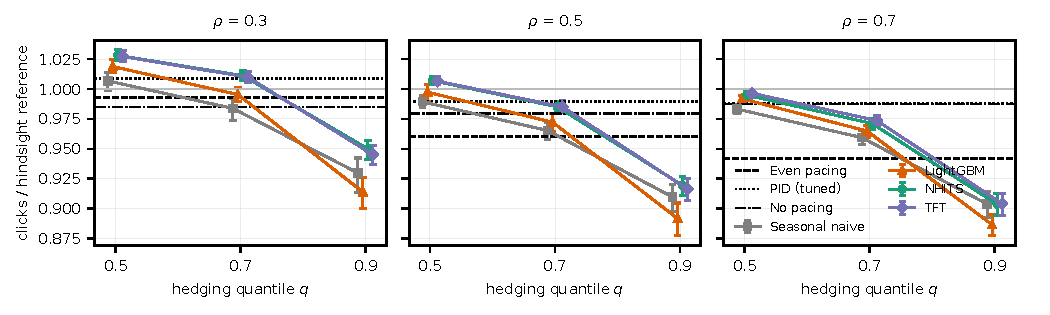
\includegraphics[width=\textwidth]{fig_hedging.pdf}
  \caption{Clicks relative to the hindsight reference as a function of the hedging quantile, with
  95\% campaign-bootstrap CIs. Horizontal lines are the forecast-free policies.}
  \label{fig:hedging}
\end{figure*}

\section{Forecasting Models}

The target is hourly campaign spend. Forecasts are issued at every hour of the test period for
the next 24 hours, using only earlier hours. All models output the quantiles
$\{0.1, 0.5, 0.7, 0.9\}$.
\begin{itemize}
  \item \emph{Seasonal naive}: empirical quantiles of the same hour on the previous seven days.
  \item \emph{LightGBM}: a direct multi-horizon model with the forecast step as a feature. It is
        trained with the quantile objective, one model per quantile. Features are spend lags,
        same-hour seasonal lags, rolling statistics, calendar phase and static campaign statistics,
        with the target normalized by the campaign's training mean.
  \item \emph{TFT} and \emph{NHITS}: \texttt{neuralforecast} models with a 168-hour input window,
        multi-quantile loss, robust scaling, historical impressions and clicks, calendar phase as
        known future inputs, and static campaign statistics.
\end{itemize}
Models are trained on the training days and early-stopped on the validation days.
Hyperparameters were fixed before evaluation and not tuned on test data. The neural models are
trained with \res{n-nn-seeds} seeds each.

% ------------------------------------------------------------------
\section{Experimental Protocol}

\begin{table}[tb]
  \caption{Forecast accuracy on the test origins, averaged over campaigns; $\pm$ is the
  standard deviation over seeds. Time is the wall-clock time to fit and forecast (neural models on
  one RTX 3070 Ti, LightGBM on an Apple M4 CPU).}
  \label{tab:forecast}
  \small\setlength{\tabcolsep}{3pt}
  \resizebox{\linewidth}{!}{\begin{tabular}{lcccccr}
\toprule
Forecaster & MASE & MASE$_{h=1}$ & MASE$_{h=24}$ & sPL$_{0.9}$ & Cov.\,80\% & Time (s) \\
\midrule
Seasonal naive & 0.917 & 0.920 & 0.908 & 0.194 & 60.6 & 0 \\
LightGBM & 0.853 & 0.810 & 0.871 & 0.185 & 71.7 & 76 \\
NHITS & 0.794 $\pm$ 0.014 & 0.719 & 0.813 & 0.158 & 75.8 & 40 \\
TFT & 0.787 $\pm$ 0.004 & 0.729 & 0.814 & 0.161 & 76.9 & 205 \\
\bottomrule
\end{tabular}
}
\end{table}

\begin{figure}[tb]
  \centering
  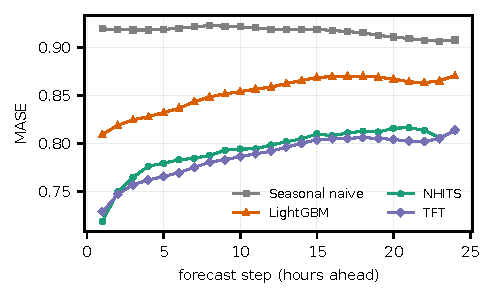
\includegraphics[width=\linewidth]{fig_horizon.pdf}
  \caption{MASE by forecast step, averaged over campaigns and seeds.}
  \label{fig:horizon}
\end{figure}



\textbf{Data.} The Criteo Attribution dataset~\cite{diemert2017attribution} contains
\res{data-impressions} impressions from \res{data-campaigns-total} campaigns over 31 days, with
the paid cost (transformed by Criteo), click and attributed conversion of each impression. The
first 21 days are for training, the next 4 for validation and the following 5 for testing.
A campaign is included if it has spend in at least 90\% of training hours. The inclusion rule
uses training data only. It keeps \res{data-campaigns} campaigns, which account for
\res{data-spend-share}\% of all spend, and gives \res{data-test-episodes} test episodes, each
replayed with \res{n-replay-seeds} seeds.

\textbf{Metrics.} Forecast accuracy is measured with MASE (scaled by each campaign's in-sample
lag-24 naive error), the scaled pinball loss sPL$_q$, the 80\% interval coverage and the
quantile-crossing rate. Pacing is measured by the ratio of clicks (and of attributed
conversions) to the hindsight reference, pooled over episodes; budget utilization (BUR); the
early-depletion rate (budget exhausted before hour 20); and the pacing volatility index (PVI),
the RMS change of $\alpha_h$ between consecutive hours.

\textbf{Statistics.} We report 95\% confidence intervals from a bootstrap over campaigns
(\res{n-bootstrap} resamples). Pre-specified paired comparisons use Wilcoxon signed-rank
tests~\cite{wilcoxon1945individual} on per-campaign click ratios, with a Holm
correction~\cite{holm1979simple} over all \res{n-comparisons} comparisons.

\textbf{Protocol.} The study protocol, including a deviation log, was written before the test
split was evaluated. All logged deviations are released, including two widenings of the PID
grid (on validation data) and intermittent GPU faults during neural training (crashed runs
produced no output and were re-run).

% ------------------------------------------------------------------
\section{Results}





\subsection{Forecast accuracy}
All four forecasters beat the in-sample seasonal-naive scale (Table~\ref{tab:forecast}). TFT
(MASE \res{fc-tft-mase}) and NHITS (\res{fc-nhits-mase}) are close and both clearly ahead of
LightGBM (\res{fc-lightgbm-mase}) and seasonal naive (\res{fc-naive-mase}). The neural models'
advantage is largest at short steps (Figure~\ref{fig:horizon}). All intervals are too narrow:
the nominal 80\% interval covers only \res{fc-tft-cov80}\% of outcomes for TFT and
\res{fc-naive-cov80}\% for seasonal naive.





\begin{figure}[tb]
  \centering
  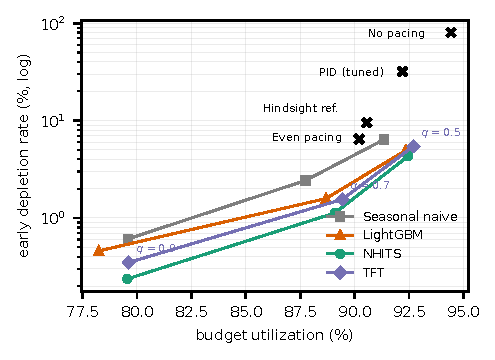
\includegraphics[width=\linewidth]{fig_tradeoff_rho0.5.pdf}
  \caption{Delivery trade-off at $\rho=0.5$: budget utilization against the early-depletion rate
  (log scale). Lines connect $q=0.5, 0.7, 0.9$ of each forecaster.}
  \label{fig:tradeoff}
\end{figure}

\subsection{Pacing outcomes}
Table~\ref{tab:pacing} and Figure~\ref{fig:hedging} summarize pacing. Throttling on the median
forecast of a neural model is the best policy at every budget level. It captures
\res{gain-even-min}--\res{gain-even-max} points more clicks than even pacing and
\res{gain-pid-min}--\res{gain-pid-max} points more than tuned PID. All
\res{cmp-nn-baselines-sig} of \res{cmp-nn-baselines-total} paired comparisons against these two
baselines are significant after Holm correction (largest adjusted $p$ = \res{cmp-nn-baselines-pmax}).
It is also far smoother: its PVI of \res{fc-pvi-min}--\res{fc-pvi-max} compares with
\res{pid-pvi-min}--\res{pid-pvi-max} for PID, and it depletes early in only
\res{fc-early-min}--\res{fc-early-max}\% of episodes, against
\res{pid-early-min}--\res{pid-early-max}\% for PID.

\textbf{The forecaster matters little.} TFT and NHITS differ by at most \res{tft-nhits-diff-max}
points of clicks; only \res{cmp-tft-nhits-sig} of \res{cmp-tft-nhits-total} of their paired
comparisons is significant. The neural models beat LightGBM by \res{nn-lgb-min}--\res{nn-lgb-max}
points (significant in \res{cmp-nn-lgb-sig} of \res{cmp-nn-lgb-total} comparisons) and seasonal
naive by \res{nn-naive-min}--\res{nn-naive-max} points. Even seasonal naive at $q{=}0.5$ is
competitive with tuned PID.

\textbf{The hedging quantile matters a lot.} Moving from $q{=}0.5$ to $q{=}0.9$ costs
\res{hedge-cost-min}--\res{hedge-cost-max} points of clicks, for every forecaster and budget level.
All \res{cmp-q09-baselines-sig} comparisons of $q{=}0.9$ policies against even pacing and PID
favor the baselines. Upper-quantile planning overstates the remaining demand, so the policy
throttles too hard and leaves budget unspent.



\subsection{The hedging trade-off}
Figure~\ref{fig:tradeoff} shows what hedging buys. At $q{=}0.9$, early depletion almost
disappears (\res{hedge-early-min}--\res{hedge-early-max}\% of episodes), but budget utilization
falls to \res{hedge-bur-min}--\res{hedge-bur-max}\%. No pacing sits at the opposite corner: it
depletes early in \res{nopacing-early-min}--\res{nopacing-early-max}\% of episodes. The median
forecast with a neural model gives the best combination of the two.

\textbf{Conversions behave differently from clicks.} No pacing captures
\res{nopacing-conv-min}--\res{nopacing-conv-max} points \emph{more} attributed conversions than
the reference, while capturing fewer clicks. One possible explanation, which we have not tested,
is that traffic early in the (dataset-relative) day converts better than it clicks. Either way, an
operator who optimizes for conversions should not assume that click-optimal pacing is also
conversion-optimal.

% ------------------------------------------------------------------
\section{Discussion}

\textbf{Practical guidance.} (i) Forecast-driven throttling is worth deploying over even pacing
and over a tuned PID. (ii) Plan against the median: the extra protection from upper quantiles is
small and expensive. If early depletion must be avoided, $q{=}0.7$ is a more balanced choice than
$q{=}0.9$. (iii) Forecast accuracy gains shrink when they reach pacing. A plausible reason, not tested here,
is that the throttle in Eq.~\eqref{eq:throttle} depends only on the \emph{sum} of the remaining
forecasts, where hourly errors can partly cancel. A cheaper model such as NHITS (\res{time-nhits}\,s versus \res{time-tft}\,s
for TFT) loses nothing here.

\textbf{Limitations.} The costs in the dataset are transformed by Criteo. The throttling model
ignores competitive responses and price effects. The test period covers five days of one
dataset. The day boundary is relative to the dataset start, not local midnight. The tuned PID
gains lie on the edge of the search grid (for example \res{pid-gains-rho0.5} at $\rho{=}0.5$),
although the validation objective is flat near the optimum. With hundreds of campaigns, small
differences become statistically significant, so we emphasize effect sizes.

% ------------------------------------------------------------------
\section{Conclusion}

On real campaign logs, forecast-driven throttling improves daily budget pacing over even pacing
and tuned PID. The main lever is the hedging quantile, not the forecasting architecture: the
median forecast works best, and upper-quantile hedging is costly. Modern neural forecasters are
the most accurate and give the best pacing, but their advantage over each other is negligible.
Future work should test these findings with bid-landscape-aware simulators and with
conversion-oriented objectives.

\bibliographystyle{ACM-Reference-Format}
\bibliography{references}

\end{document}
